%!TEX root = ../../exa-ma-d7.1.tex
%\chapter{Work Package 3: Solvers for Linear Algebra \& Multiphysics}
%\label{chap:wp3}

\section{Objectives \& Context}
% • Which Exa-MA bottlenecks (B#) WP3 addresses  
% • Role in overall strategy (Krylov solvers, domain decomposition, mixed precision)  
% • List of key tasks T3.1–T3.3

We first intend to design novel or improved numerical kernels that are mostly agnostic of the
underlying models (e.g., PDE) and approximation techniques (e.g., FEM) for the solution of linear
systems. The envisioned solution techniques are generic in the sense that they do not depend on the
way the function f is represented (e.g., matrix or implicit access to f in the linear case). To reduce the
computational complexity, memory footprint and data movement, techniques such as communication
avoiding/hiding, mixed arithmetic and data compression (e.g., low-rank approximations) will be
exploited. The second objective is to fully exploit the extreme parallelism enabled by the forthcoming
platforms to design coupled physic solvers that rely on state-of-the-art optimized mono-physics
solvers.

We recall below the corresponding tasks as described in the original proposal. 



\subsubsection*{T3.1 Domain decomposition methods with subspace-correction}

 To enhance the scalability of
multilevel domain decomposition methods, we will investigate theoretically and experiment their
robustness with respect to inexact setups and applications of the preconditioner that might arise for
instance from mixed arithmetic calculation, inexact local solves, low rank approximations. The
validation of these studies will be conducted primarily in the HPDDM library but could also benefit
others such as Composyx.
.
\subsubsection*{T3.2. Exploiting data-sparsity, multiple precision and data compression}
\paragraph*{T3.2.1 Modular, composable mixed precision Krylov solvers. }

Subspace Krylov exhibits appealing
features enabling the use of mixed precision arithmetic in different computational steps that might be
computed by different numerical variants in a modular manner. To guarantee the final numerical
quality of the computed solution novel modular, analyses must be developed for enabling composable
parallel implementations of these subspace solvers (in close collaboration with PC2).

\paragraph*{T3.2.2 Decoupling the data representation from the arithmetic: the variable accuracy paradigm}

The variable accuracy paradigm is a promising avenue to control the memory footprint and the
volume of communication by decoupling the data representation from the arithmetic, while ensuring a
user-prescribed accuracy. Some analysis must be developed to guarantee the numerical quality of the
computed solutions; this will enable robust implementations of the numerical solvers (in close
collaborations with PC2) fully exploiting the underlying features (memory and processing units) of
modern computing architectures.
\paragraph*{T3.2.3 Precision auto-tuning tools}
 Precision auto-tuning tools provide mixed precision versions of
numerical codes, taking into account accuracy requirements on the results. New algorithms must be
proposed to improve precision auto-tuning performance and extend it to arbitrary precision.
Furthermore, new methodologies must be developed to perform autotuning of both numerical formats
and performance parameters in coupled physics simulations as addressed in Task 3.3.2.
\paragraph*{T.3.2.4 Silent errors in solution techniques}
 The objective of this task is to study and design silent
error detection and hopefully correction that might appear at scale. These evaluations will either be
tailored to the intrinsic properties of the numerical schemes or based on statistical techniques.

\subsubsection*{T3.3 Adaptive solution strategies for exascale multiphysical and multiscale models}
\paragraph*{T3.3.1 Many multiphysics problems may be recast as saddle point problems}

 The task will
consist of investigating the parallel efficiency of domain decomposition methods for the solution of
saddle point problems for coupled multiphysics problems.

\paragraph*{T3.3.2 Exascale resolution for simulations in partitioned coupling}

 The task will consist of the
automatic tuning of performance parameters appearing in the partitioned coupling between
exascale-ready software components. Such parameters (coupling strengths, path between physics,
adaptive internal convergence criteria…) are intended to be handled through a joint strategy with the
auto-tuning work from Task 3.2.3.



\section{Scientific Advances}

%IMAGES si vous en avez!! 


 \subsection{ 
 Advance 1 (T3.1): Domain decomposition methods with subspace-correction 
 }
 %These de Tom (Frédéric et Theo) \\
 \subsubsection{Stability with respect to approximate subsolves and round-off errors}
\label{sec:wp3:T31:ddmroundoff}
The PhD subject of Tom Caruso (advisors: P.~Jolivet, T.~Mary, F.~Nataf and P.H.~Tournier) supported by Exama-NumPEx is concerned with domain decomposition preconditioners, the Additive Schwarz method (ASM) with GenEO (Generalized Eigenproblems in the Overlap) coarse space, to solve large, sparse symmetric positive definite (SPD) problems. 
Through libraries such as HPDDM, these preconditioners have already been efficiently parallelized in their numerical implementations. 
However, they still require expensive, in time and memory, linear algebra operations in each local subdomain. 
Motivated by the emergence of fast low precision arithmetic in hardware, the aim of his work is to reduce the computation time and memory foot-print of the ASM-GenEO using mixed precision. 
To do this, it is necessary to identify the sensitivity of these operations to perturbation and propose an actionable criteria for selecting the appropriate precision for each local subdomain.
Using the Fictitious Space Lemma, a perturbation theory for the preconditioner and bound the worst-case loss of efficiency of the preconditioner are derived. The results show that  precision selection is guided by the local matrix condition number. 
Moreover, using FreeFEM, petsc4py, and HPDDM libraries, the theoretical bounds are compared to numerical behaviour of the perturbed preconditioner and are thus validated. 

These results therefore suggest that preconditioners can be constructed in mixed precision while effectively controlling the loss of efficiency. In order to apply these theoretical results and enhance the scalability of
multilevel domain decomposition methods, we will investigate theoretically and experiment their
robustness with respect to inexact setups and applications of the preconditioner that might arise for
instance from mixed arithmetic calculation, inexact local solves, low rank approximations. The
validation of these studies will be conducted primarily in the HPDDM library but could also benefit
others such as composyx. 


 In this respect, this work is also very closely related to \S~\ref{sec:wp3:T32}. 


 \subsubsection{HPDDM for sensitivity analysis}
 
The ability to apply the transpose of a preconditioner is particularly valuable for sensitivity analysis and adjoint-based computations, where one needs to propagate perturbations backward through the system. This capability ensures consistency between forward and adjoint solves, improving the reliability of derivative-based optimization. This feature was recently added to HPDDM. For the coarsest level, efficiency has been further enhanced by the use of analysis by block in MUMPS, which exploits the block structure of the system to reduce the cost of symbolic factorization and accelerate the setup phase of the direct solver. Finally, for unsymmetric saddle-point systems, techniques originally developed for least-squares problems—such as normal equation reformulations—have been adapted to handle the indefiniteness and non-symmetry, providing robust and scalable convergence even in challenging PDE-constrained optimization and computational fluid dynamics. 
 
 

 \subsubsection{Domain decomposition methods for non-SPD problems}
  \label{sec:wp3:T31:nonSPD}
For symmetric positive definite (SPD) problems, provably scalable domain decomposition methods are known, even for heterogeneous media and complex PDE systems, such as elasticity problems, in particular thanks to the GenEO preconditioner~\cite{Spillane:2014:ASC, Dolean:2015:IDDSiam}. In a series of recent works, this approach has been extended to several types of non-SPD problems.

A first class of non-SPD problems are saddle point problems whose discretization cannot be written as both symmetric and positive definite; it may be symmetric but not positive definite, or positive definite but not symmetric. For these problems, the GenEO method has been used in~\cite{nataf:hal-02343808} and~\cite{brunelli:hal-05123311} to construct two-level domain decomposition preconditioners for both the primal problem and the Schur complement problem (obtained by eliminating the primal unknown from the system). The novelty of our analysis and construction lies in the combined use of domain decomposition methods of Schwarz type and Neumann–Neumann/FETI type. It is now possible to solve highly heterogeneous nearly incompressible elasticity problems (such as steel-rubber) with a continuous pressure discretization, involving one billion degrees of freedom on 16,000 compute cores.

An algebraic approach has been developed in~\cite{nataf:hal-04536547} to provide a generic way of constructing spectral coarse spaces to be used in two-level domain decomposition preconditioners, that is valid for a large class of non-SPD problems. To our knowledge, this is the first mathematical theory for the restricted additive Schwarz (RAS) method with inexact local solves, such as provided by ILU0 factorizations, the default DD solver in PETSc. 



 \subsection{  Advance 2 (T3.2): Exploiting data-sparsity, multiple precision and data compression}
\label{sec:wp3:T32}
 \subsubsection{ 
 T3.2.1 Modular, composable mixed precision Krylov solvers. 
 }
  Subspace Krylov exhibits appealing
features enabling the use of mixed precision arithmetic in different computational steps that might be
computed by different numerical variants in a modular manner. To guarantee the final numerical
quality of the computed solution novel modular, analyses must be developed for enabling composable
parallel implementations of these subspace solvers (in close collaboration with PC2).

%(Luc + Pierre ) stage d'Erik 

During the master internship of Erik Fabrizzi, funded by Exama-NumPEx, we have been working on a high-performance implementation of Augmented GMRES. Augmented GMRES with mixed precision is an iterative Krylov subspace method designed to accelerate the solution of large, sparse linear systems while reducing computational cost. The augmentation step incorporates approximate solutions or precomputed subspaces (e.g., from deflation or previous solves) to enrich the Krylov basis, improving convergence. By exploiting mixed precision arithmetic—using low precision for operations such as matrix-vector products while retaining higher precision for critical steps such as orthogonalization and residual correction—the method balances efficiency and accuracy. 

 \subsubsection{ T3.2.2 Decoupling the data representation from the arithmetic}

The variable accuracy paradigm is a promising avenue to control the memory footprint and the
volume of communication by decoupling the data representation from the arithmetic, while ensuring a
user-prescribed accuracy. Some analysis must be developed to guarantee the numerical quality of the
computed solutions; this will enable robust implementations of the numerical solvers (in close
collaborations with PC2) fully exploiting the underlying features (memory and processing units) of
modern computing architectures. 

%(Luc + Manu + Pierre + Théo) stage de Alexandre même si tâche commencée pas à l'endroit prévu 

During the master internship of Alexandre Tabouret, which will be followed up by a Ph.D. thesis starting in October 2025, we have been investigating the combination of relaxed GMRES and adaptive sparse matrix-vector products. Relaxed GMRES is a variant of the GMRES in which the accuracy of matrix–vector products or inner solves is reduced dynamically as iterations progress, since later iterations require less precision to maintain convergence. This relaxation lowers computational cost without significantly impacting accuracy. Adaptive SpMV (sparse matrix–vector multiplication) complements this idea by adjusting arithmetic precision or sparsity handling based on error tolerances or convergence state. Together, relaxed GMRES with adaptive SpMV leverages variable precision and workload reduction to accelerate iterative solvers while preserving numerical stability.

\subsubsection{ 
T3.2.3 Precision auto-tuning tools
} 

Precision auto-tuning tools provide mixed precision versions of
numerical codes, taking into account accuracy requirements on the results. 
% ajout par Frédéric suite au commentaire de @Christophe (2025-10-08-15:06) ...
Achieving optimal performance in numerical computations often hinges on aggressively quantizing arithmetic and data to low-precision formats or rigorous rounding error analysis to retain numerical accuracy. The PROMISE (PRecision OptiMISE) software provides a task-specific validation using  \href{https://cadna.lip6.fr/}{CADNA}  (https://cadna.lip6.fr) for automated precision tuning, enabling a balance between computational efficiency and numerical fidelity. PROMISE allows for customized precision formats to examine the low-precision potential in a suite of numerical algorithms for performance gains, offering actionable insights into selecting optimal precision levels for diverse algorithms.
% ... fin de l'ajout
It also has the particularity to combine precision auto-tuning and numerical validation thanks to stochastic arithmetic implemented in the CADNA library. 
First versions of PROMISE 
could provide transformed user codes that mix FP64, FP32 and FP16 numerical formats. 
With the emergence of various new numerical formats, it became necessary to extend PROMISE to arbitrary precision. This task has been carried out with
Xinye Chen, post-doc in Sorbonne Université supported by Exama-NumPEx. 
PROMISE has been combined with the \href{https://github.com/oprecomp/FloatX}{FloatX} library that provides user-defined types with both an arbitrary mantissa length and an arbitrary exponent length. 
This has implied the extension of FloatX to enable the use of mathematical functions with arbitrary precision arguments. 
From the expected accuracy in the results and a list of native or emulated numerical formats, PROMISE automatically transforms an input code into a mixed precision version using the types in the given list. This new version of PROMISE has been successfully tested on various numerical analysis
codes and Machine Learning codes, including codes from the Rodinia Benchmark suite, and has shown the potential for using low precision settings. 
Besides, the codes tested with PROMISE form a publicly available set of benchmarks for precision auto-tuning tools.

%New algorithms must be proposed to improve precision auto-tuning performance and extend it to arbitrary precision.
%Furthermore, new methodologies must be developed to perform auto-tuning of both numerical formats and performance parameters in coupled physics simulations as addressed in Task 3.3.2.
%(Fabienne) post doc de Xinye 


\subsubsection{ 
T.3.2.4 Silent errors in solution techniques
}
 The objective of this task is to study and design silent
error detection and hopefully correction that might appear at scale.  
%These evaluations will either be tailored to the intrinsic properties of the numerical schemes or based on statistical techniques.
Hence, we have investigated how to protect numerical iterative algorithms from all types of errors that can strike at scale: fail-stop errors (a.k.a. failures) and silent errors, striking both as computation errors
 and memory bit-flips. We have combined various techniques: detectors for computation errors,
  checksums for memory errors,  and checkpoint/restart for failures.  The objective is to minimize the expected time per iteration of the algorithm. We designed a hierarchical pattern that combines and interleaves all these fault-tolerance mechanisms, and we determined
  the optimal periodic pattern that achieves this objective. We instantiated these results for the performance analysis of the Preconditioned Conjugate Gradient (PCG) algorithm, reporting several scenarios where the optimal pattern dramatically decreases the overhead due to error mitigation.

  This work was conducted with an internship student, Alix Tremodeux, co-advised by the Roma and Concace teams~\cite{tremodeux:hal-04872041}, and it led to a publication that will appear in the International Journal of High-Performance Computing Application (IJHPCA)~\cite{tremodeux:hal-05234063}.

%(Anne ) stage d'Alix article publié suite au stage ++ 
 
 \subsection{ 
T3.3 Adaptive solution strategies for exascale multiphysical and multiscale models
 }

\subsubsection{ 
 T3.3.1 Many multiphysics problems may be recast as saddle point problems
 }
 \label{sec:wp3:T331}
  The task will consist of investigating the parallel efficiency of domain decomposition methods for the solution of saddle point problems for coupled multiphysics problems.

  Lukas Spies has started his postdoctoral work in March 2025. He has developed a parallel FreeFEM script that allows for non-matching grids at the interface between two domains. The coupling scheme, analyzed in~\cite{japhet_robin_2014}, is based on the use of Robin interface conditions. An extra level of parallelism comes from the domain decomposition solver in each domain. The global coupled system has a saddle-point structure. A study of various preconditoning strategies is underway. The flexibility and effectiveness of a parallel FreeFEM script is a great asset for numerical tests. 

%(Lukas) 

\subsubsection{ 
T3.3.2 Exascale resolution for simulations in partitioned coupling
}
 The task will consist of the
automatic tuning of performance parameters appearing in the partitioned coupling between
exascale-ready software components. Such parameters (coupling strengths, path between physics,
adaptive internal convergence criteria…) are intended to be handled through a joint strategy with the
auto-tuning work from Task 3.2.3. This task has recently been started with the work of Utpal Kiran at CEA and supported by Exama-Numpex. 

 %(Utpal)


\section{Application Showcase}
% \input{chapters/applications/specs/app-hpddm-solver-1}  
% \input additional app specs as needed
The work by Parolin and Nataf mentioned in \S~\ref{sec:wp3:T31:nonSPD} has been successfully applied to convection-diffusion problems and to time-harmonic acoustic propagation problems~\cite{dolean:hal-05241475}. As an illustration of the efficiency of the approach, we provide some weak scaling results extracted from~\cite{dolean:hal-05241475} on the 3D Cobra cavity problem, see Table~\ref{tab:weak_scaling_cobra} and Figure~\ref{fig:solutions_cobra}. 

\begin{table}[H]
    \scriptsize
\begin{center}
\begin{tabular}{cccc}
Nb CPUs & Matrix size & Iterations one-level & Iterations two-level~\cite{nataf:hal-04536547} \\
\hline
32 & 473004   & 51   &  8 \\
108 & 1761164  & 157  & 10 \\
256 & 4140366  & 359  & 14 \\
500 & 8431281  & 432  & 16 \\
864 & 13927097 & 942  & 34 \\
1372 & 18879654 & 1055 & 44 \\
2048 & 32848020 & 3711 & 60 \\
2916 & 44520439 & 3398 & 74 \\
\end{tabular}
\end{center}
    \caption{
		Weak scaling experiment for the cobra cavity test case.
    }\label{tab:weak_scaling_cobra}
\end{table}
\begin{figure}[H]
    \centering
	{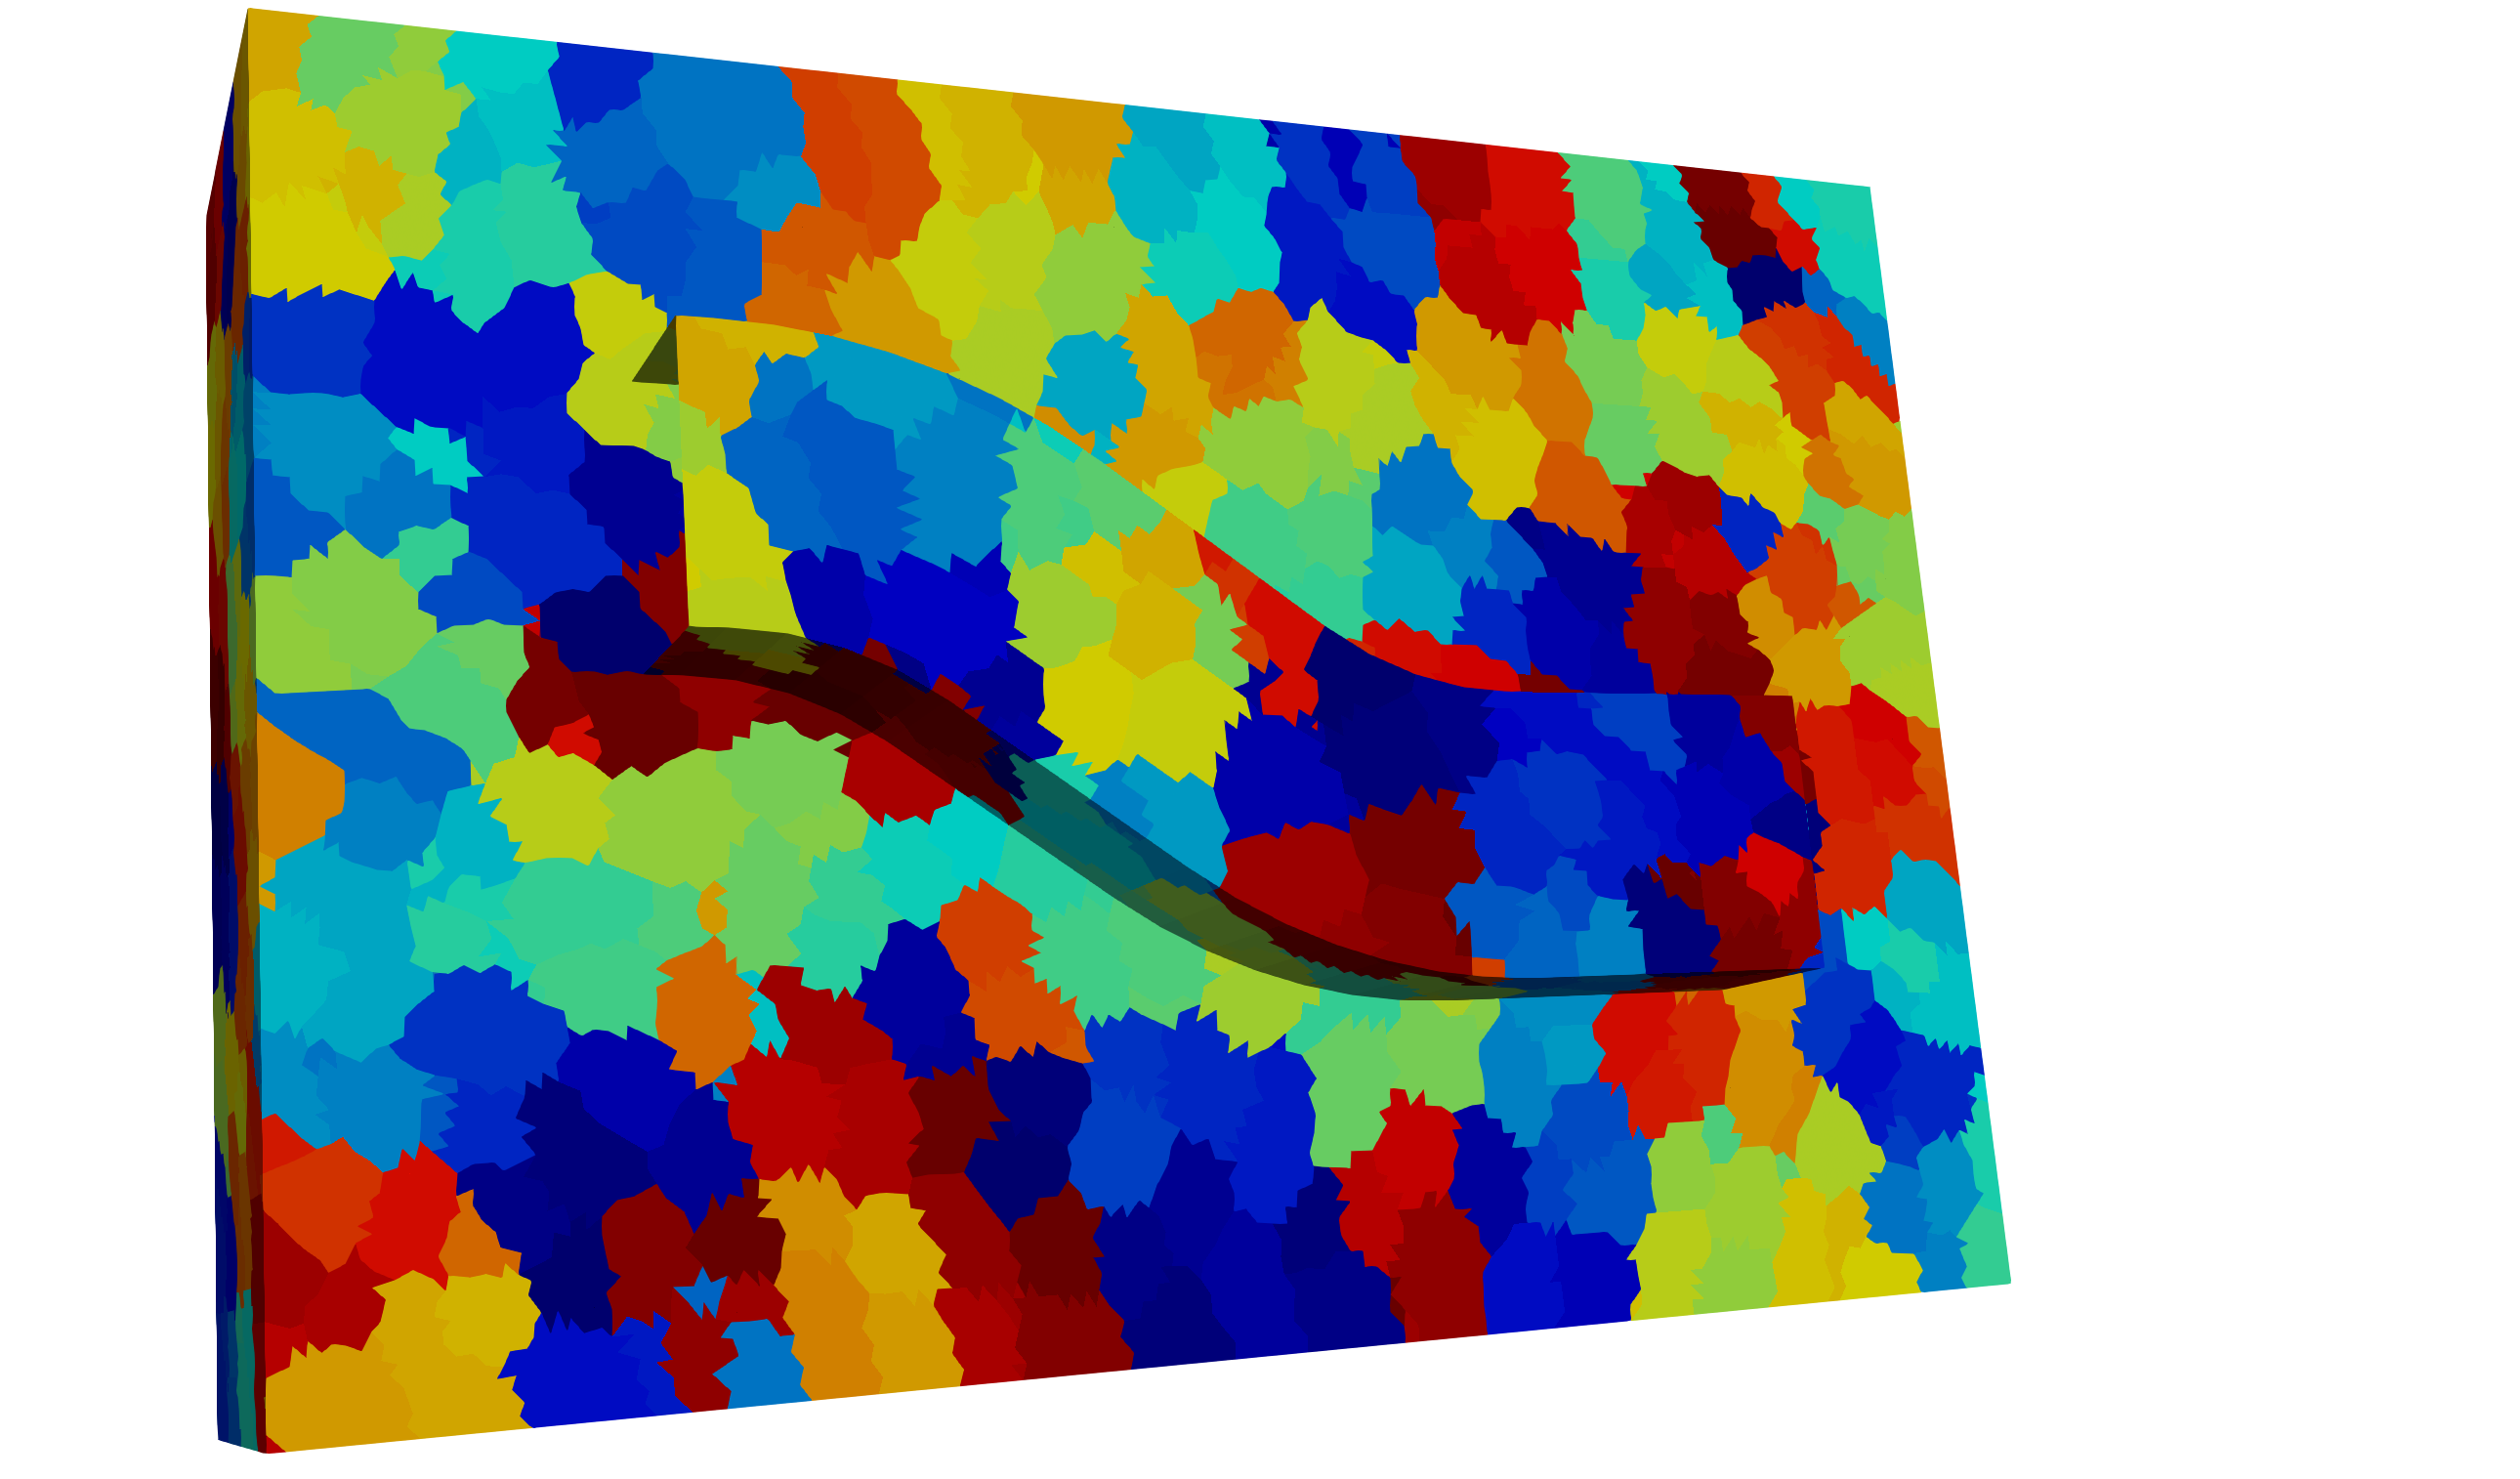
\includegraphics[width=0.48\textwidth,clip=true,trim=7cm 0cm 7cm 0cm]{./graphics/wp3/cobra_mesh_2.png}}
	{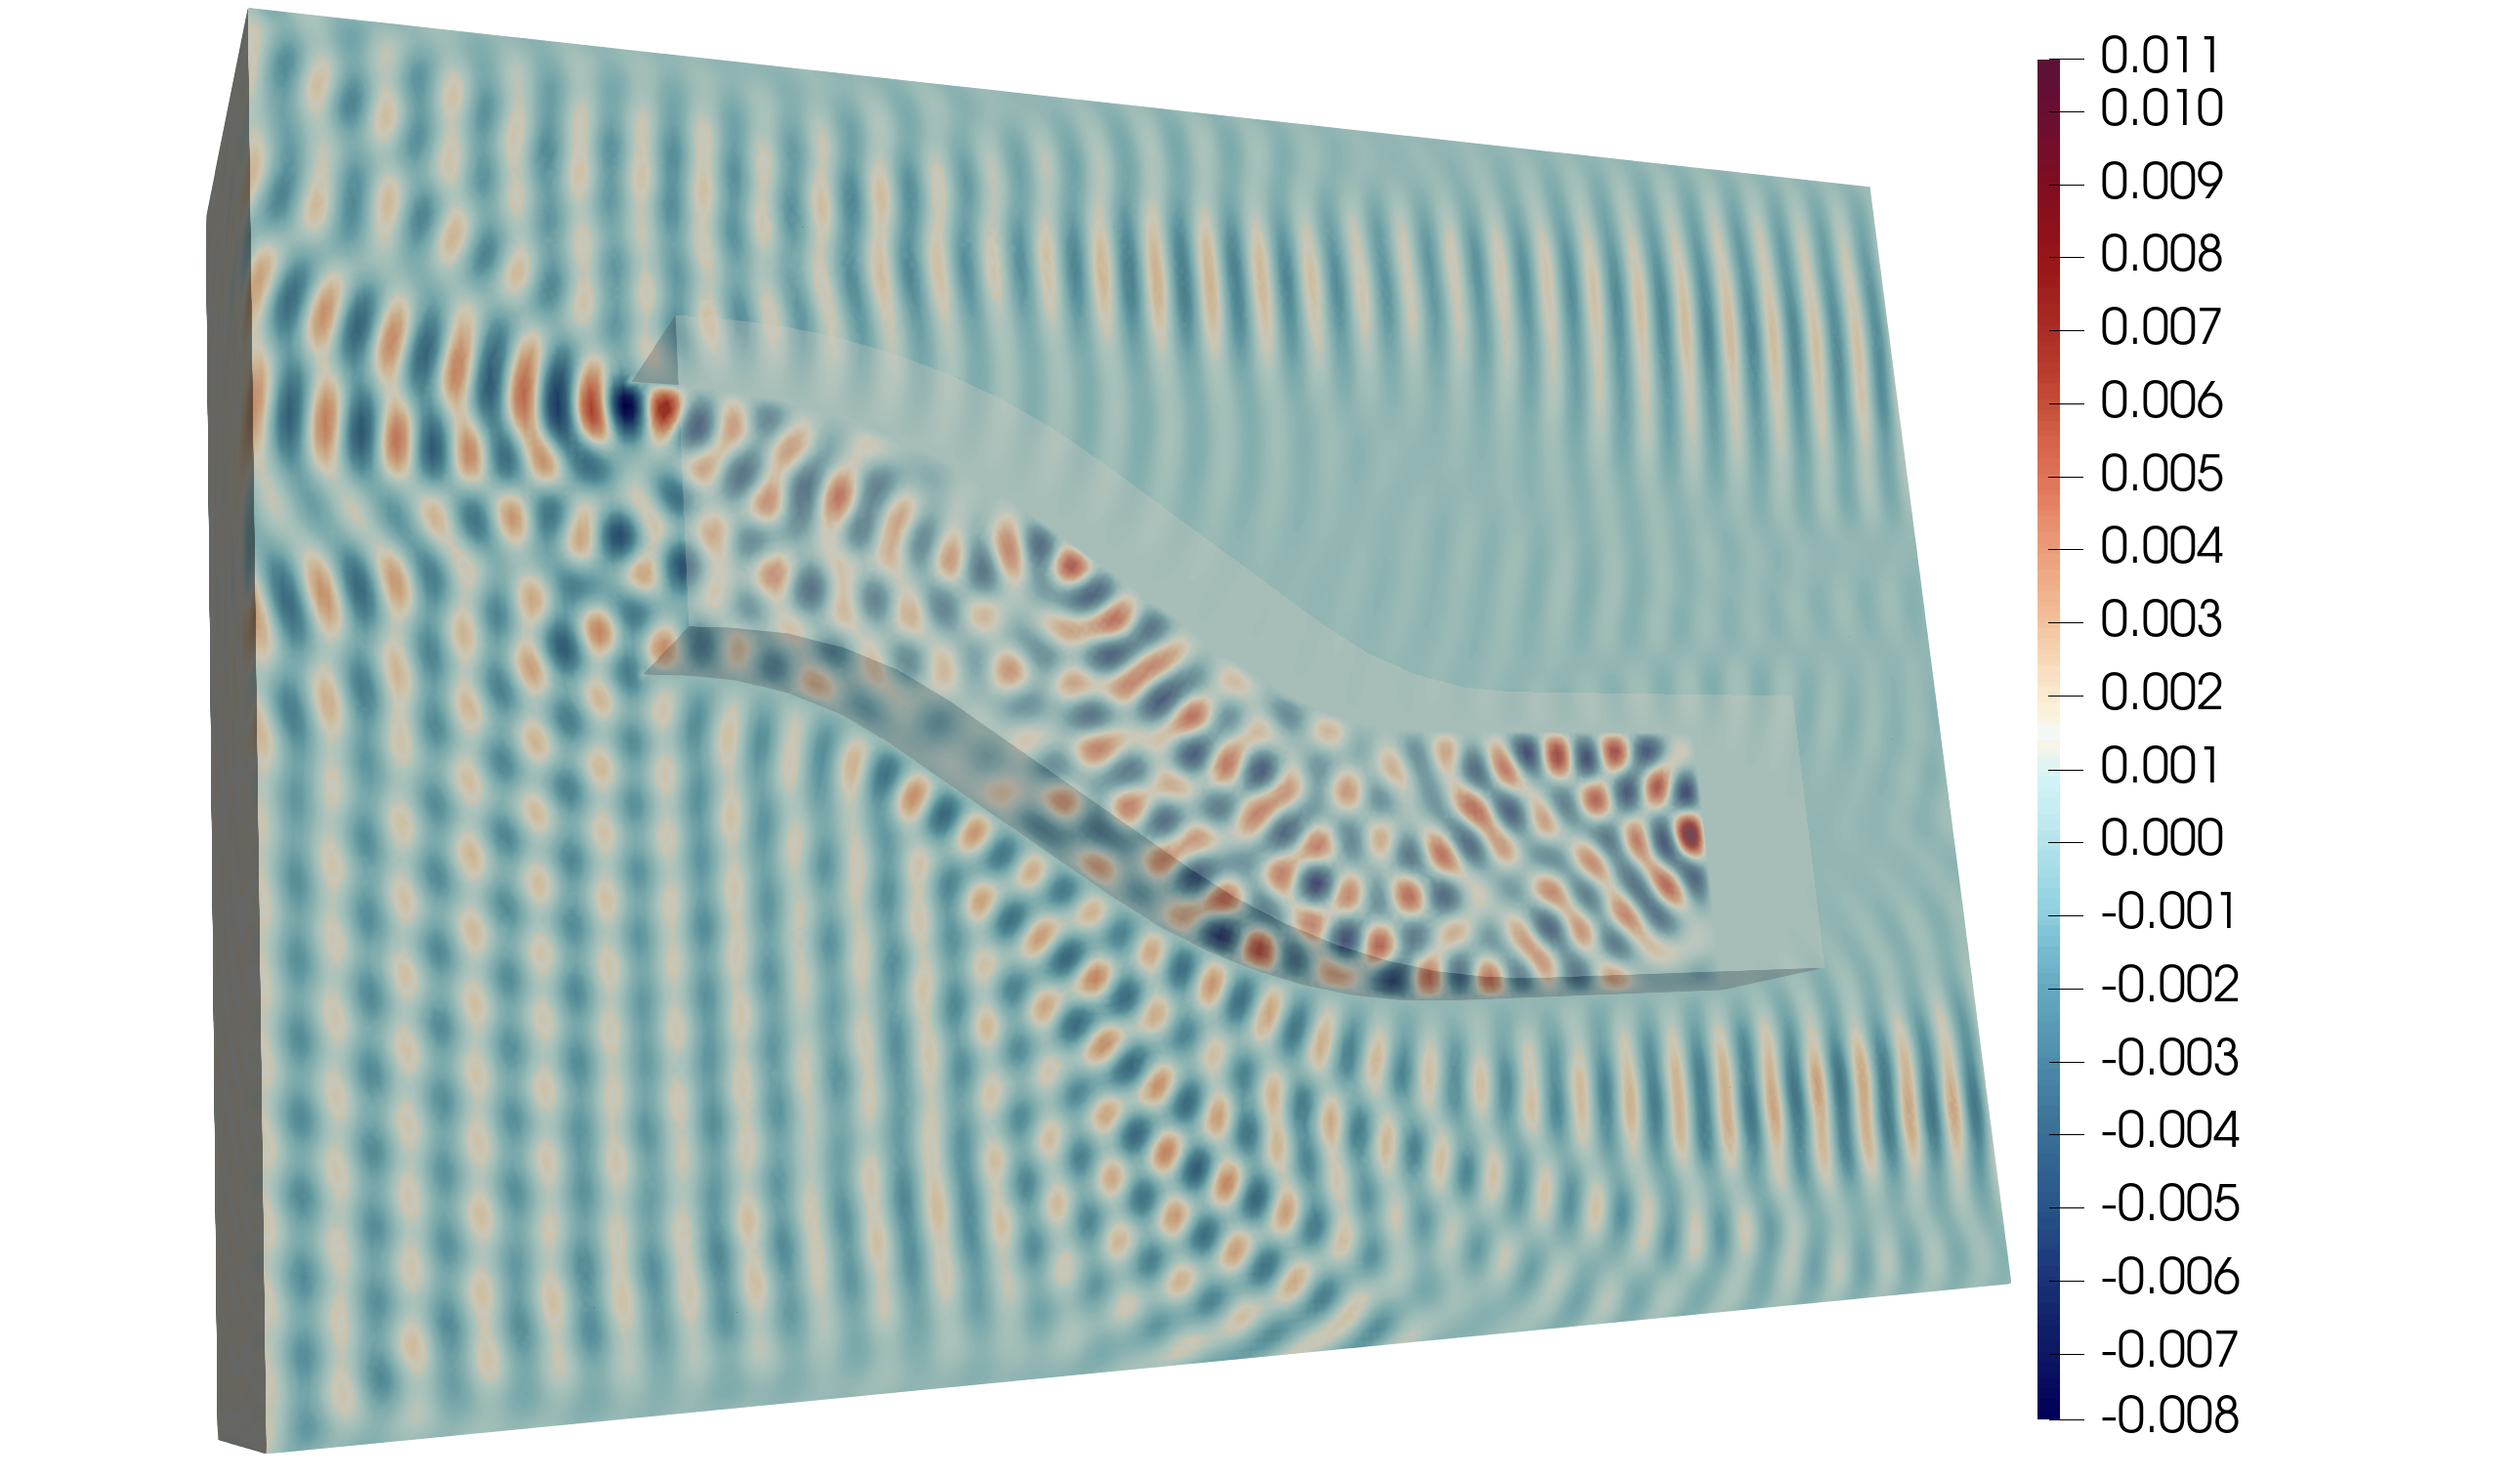
\includegraphics[width=0.48\textwidth,clip=true,trim=7cm 0cm 7cm 0cm]{./graphics/wp3/cobra_real.png}}
	\caption{
		Partitioning of the cobra cavity domain into 2916 subdomains (left) and real part of the total field (right) for wavenumber $k = 360m^{-1}$. 
    }\label{fig:solutions_cobra}
\end{figure}
Note that the method has also been successfully applied to the generation of synthetic high fidelity data for medical imaging problems, not shown here. 


\section{Software Framework Contributions}
 • HPDDM: new releases this year (from version 2.3.1 to 2.3.5), support from applying the transpose of preconditioners, preliminary support for subdomain computations on (NVIDIA) GPU, interface to MUMPS ICNTL(15), multiple fixes for non-symmetric saddle-point systems
 
 • PETSc enhancements: new releases this year (from version 3.22 to 3.24), interface to MUMPS ICNTL(15) used by HPDDM, new automatic Fortran binding generation for better interoperability between C, C++ and Fortran, new API PCMatApplyTranspose() and PCShellSetMatApplyTranspose() used by HPDDM
 
 • Composyx: % (en attente de Luc)
 This work focuses on developing robust and high-performance solutions for large sparse linear systems on modern, increasingly heterogeneous computing platforms. It targets the optimization of domain decomposition algorithms within the Composyx framework, combining direct and iterative methods to improve scalability and accuracy. The approach integrates state-of-the-art libraries for dense and sparse linear algebra and efficient domain partitioning to ensure computational efficiency. Recent work has allowed consolidating performance portability for both MPI + threads and MPI + GPU setups. An Exa-MA engineer has been hired and started on October 1, 2025.
 
 • %Mixed-precision module: PROMISE (Fabienne)
The work carried out in Task 3.2.3 (precision auto-tuning tools) has enabled to extend PROMISE to arbitrary precision emulated formats. 
From an accuracy requirement and a list of native or emulated numerical formats, PROMISE can provide a mixed precision version of C/C++ code using those formats.

\section{Preliminary Benchmarks \& Trends}
We are in close connection with the activities of the work-package WP7 where benchmarks related to domain decomposition methods are shown. 
% • Solver scaling placeholder  
% • Mixed-precision speedups placeholder  
% • Regression test pass-rate placeholder

\section{Roadmap \& Next Steps}

%a ecrire dans chaque section, résumer pour chaque section en faisant des références au texte plus haut.

In Task~3.1, the next step in \S~\ref{sec:wp3:T31:ddmroundoff} related to domain decomposiiton methods with mixed precision is to assess their performance gains using single precision in well-behaved subdomains and double precision in badly behaved subdomains. As for \S~\ref{sec:wp3:T31:nonSPD}, we intend to test this new framework on low frequency Maxwell problems which are slightly non positive and which appear in many engineering applications. 


Task 3.2.3 (precision auto-tuning tools) will require 
more results analysis. For instance, for linear system solving, the link between iterative refinement and precision tuning can be explored.
Next steps include the development of new methodologies to perform auto-tuning of both numerical formats and performance parameters in coupled physics simulations as addressed in Task 3.3.2.

Task~3.3.1 in \S~\ref{sec:wp3:T331} will be extended to demanding problems both in terms of problem dimension and in terms of physics. 

% • Deliverables D3.x to complete by Mxx  
% • New solver apps to integrate into WP7 CI/CD  
% • Dependencies on WP7 infrastructure (containers, ReFrame)  







